\documentclass[a4paper,12pt]{diplom}
% \usepackage[latin1]{inputenc}
% \usepackage[utf8]{inputenc}
\inputencoding{utf8} % Кодировка вашего файла


\usepackage{paratype} % Шрифты (можно отключить, если дает ошибку)
%% Немного увеличим шрифт в математическом режиме, чтобы соответствовать размерам Paratype-шрифтов
\DeclareMathSizes{12}{13.4}{11}{10}

\usepackage[left=3cm,right=2cm,top=2cm,bottom=2cm]{geometry} % Размеры полей
\usepackage[onehalfspacing]{setspace} % Полуторный интервал
%\renewcommand{\baselinestretch}{1.25} % Полуторный интервал
\usepackage{indentfirst} % Абзацный отступ в начале разделов
\setlength{\parindent}{1.25cm} % Величина абзацного отступа

\usepackage[pdftex]{graphicx} % Для вставки изображений
\usepackage{array} % Для таблиц
\usepackage{booktabs} % Для красивых таблиц 
\usepackage{tikz} % Рисунки с помощью TikZ
\usepackage[linesnumbered,lined,ruled]{algorithm2e} % Для оформления псевдокода
%\usepackage{algorithm} % Альтернатива оформления псевдокода
%\usepackage{algpseudocode} % Альтернатива оформления псевдокода
\usepackage{listings} % Оформление листингов программ
\usepackage{icomma} % Удаляем тонкий пробел после запятой в мат. режиме
\usepackage{centernot}
\usepackage[figure,table]{totalcount}

% Если на нумерованную формулу нет ссылки в тексте,
\mathtoolsset{showonlyrefs} % то она становится ненумерованной

% microtype улучшает распределение символов в строке
\usepackage{microtype}  % Можно отключить, если возникают ошибки компиляции

% Формируем PDF с полноценными перекрестными ссылками
\usepackage[unicode, pdfborder={0 0 0}, pdfstartview=FitV]{hyperref}

% Часто используемые макросы
\newcommand{\N}{\mathbb{N}}  % Множество натуральных чисел
\newcommand{\Z}{\mathbb{Z}}  % Множество целых чисел
\newcommand{\R}{\mathbb{R}}  % Множество действительных чисел
\DeclareMathOperator{\sgn}{sgn} % Знак числа
\DeclareMathOperator{\M}{\mathsf{M}} % Матожидание
\newcommand{\from}{\colon} % Двоеточие в определении функции. Пример: $f \from \R \to \N$.
% Заменяем англоязычные обозначения на русские
\renewcommand{\le}{\leqslant}
\renewcommand{\leq}{\leqslant}
\renewcommand{\ge}{\geqslant}
\renewcommand{\geq}{\geqslant}
\renewcommand{\emptyset}{\varnothing}
\renewcommand{\epsilon}{\varepsilon}


%%%%%%%%%%%%%%%%%%%%%%%%%%
% Конец преамбулы
%%%%%%%%%%%%%%%%%%%%%%%%%%

% ==================== Титульный лист ====================

\begin{document}

% Содержимое титульного листа

%\LetterHead{Минобр...}
\Kafedra{Кафедра дискретного анализа}

% Зав. кафедрой
\ZavKaf{Заведующий кафедрой,\\ д.\,ф.-м.\,н., профессор}{В.\,А.~Бондаренко}
% Если это курсовая работа и виза зав. каф. не нужна, раскомментируйте следующую строку
%\Kursovaya

% Вид работы: Курсовая работа, Выпускная квалификационная работа, 
\DocumentType{\large Выпускная квалификационная работа}

% Название дипломной работы
\Title{\begin{Large}\bfseries Методы обратной свертки в задачах \\ космической физики\end{Large}}

% Направление подготовки
\Napr{по направлению\\ 01.04.02 Прикладная математика и информатика}

% Руководитель
\Chief{Научный руководитель\\ к.\,ф.-м.\,н., доцент}{Ю.\,В.~Богомолов}

% Автор
\Author{Студент группы ИВТ-21МО}{А.\,В.~Ющенко}

%\City{Ярославль}
%\Year{2017}


\maketitle
\chapter*{Реферат}

Объем \total{page} с., \total{chapternum} гл., \totalfigures\ рис.,
\total{tablenum} табл., \total{bibnum} источников, \total{appnum} прил.

\medskip

Ключевые слова: \textbf{Обратная свертка, Unfolding, SVD}

\medskip

На сегодняшний день электронные измерительные приборы используются повсеместно, почти не осталось отраслей, где бы не использовались цифровая аппаратура. 
Однако, результаты измерений могут быть искажены и трансформированы из-за множества факторов. Одной из областей, нуждающихся в поиске истинных 
значений, до искажения, является космическая физика. Также усложнением задачи являться то, что нужно восстанавливать многомерные измеренные спектры 
космических частиц. Для решения данной задачи в работе предлагается рассмотреть модификации метода SVD (Singular Value Decomposition) подхода для 
решения задачи обратной свертки.


\tableofcontents[Содержание]


\chapternonum{Введение}

В ходе проведения экспериментов, одной из возможных целей для анализа может служить распределение наблюдаемой случайной величины. Однако, 
используя для регистрации измерительные приборы, неизбежно происходит искажения исходного спектра. Это может объясняться внешними воздействиями 
или влиянием конечного разрешения аппаратуры. При анализе подобных результатов измерения, будет затруднена или даже невозможна интерпретация 
полученных данных. А так же может быть затруднен сравнительный анализ данных, полученных с использованием разной аппаратуры в отличающихся 
условиях. Обладания знаниями о возможном искажении, можно получить функцию с двумя переменными, описывающую отклик детектора. Для получения 
исходного спектра необходимо выполнить свертку этой функции с истинным распределением. В общем случаи, это приводит к интегральному уравнению.
Самым результативным способом на сегодняшний день, является гистограммный подход, требующий дискретизацию множества значений случайной величины 
и последующем решении системы линейных уравнений, однако, "наивное" решение данной задачи, является неустойчивой к малым колебаниям исходной 
системы, что, в свою очередь, приводит большим статистическим ошибкам.

Данный подход решения задачи называется задачей анфолдинга (от англ. Unfolding) или обратной свертки. Зная о дефектах 
приборов можно создать математическую модель, с помощью которой построить качественные оценки распределений и использовать их для решения 
задачи обратной свертки. При таком подходе необходимо разбить множество допустимых значений на интервалы и посчитать количество попаданий 
в каждый интервал (гистограмму), далее следуют определить вероятности попадания истинного распределения в i бин (интервал) 
при условии, что измеренная частица попала в j бин. На основе этих данных строится матрица миграций и уже сверка, измеренного спектра с ней, 
даст оценку истинного распределения.

Одним из способов решения задачи анфолдинга, может быть SVD (Singural Value Decomposition) алгоритм. Главным его достоинством является
возможность учитывать характер исходного распределения, например, непрерывность или гладкость. Данный подход называется регуляризационным
и широко применяется для решения одномерной задачи.

При работе с космическими частицами, физическая величина может оказаться многомерной, в данный работе рассмотренны частицы со следующими
характеристиками: направление и жесткость. Для подобных задач стандартный методом регуляризации не подходит, так как он может учитывать
только гладкость соседних бинов, а их структура является плоской, то есть, многомерный случай рассматривается, как последовательный набор
одномерных сечений, что не позволяет учитывать соседство в n-мерном случаи.

В данной работе исследуется вопрос решения многомерной задачи обратной свертки методом регуляризации, а так же доработка и изучение уже
существующего метода предложенного в работе \cite{SvdHocker}.



\chapter{Решения задачи обратной свертки}
\section{Постановка задачи}

Распределение, измеренной наблюдаемой величины, может хранится в векторе $m$ размерности $n_{m}$, где i-я координата вектора содержит 
количество элементов, попавших в соответствующий бин гистограммы. На измерение влияет конечное разрешение измерительной аппаратуры или 
внешние помехи, поэтому каждое событие из истинного распределения может оказаться соседних бинах или вообще вне диапазона. 
Предположим, что мы можем смоделировать процедуру измерения этой наблюдаемой (например, с помощью методов Монте-Карло). 

\begin{figure}[!ht]
   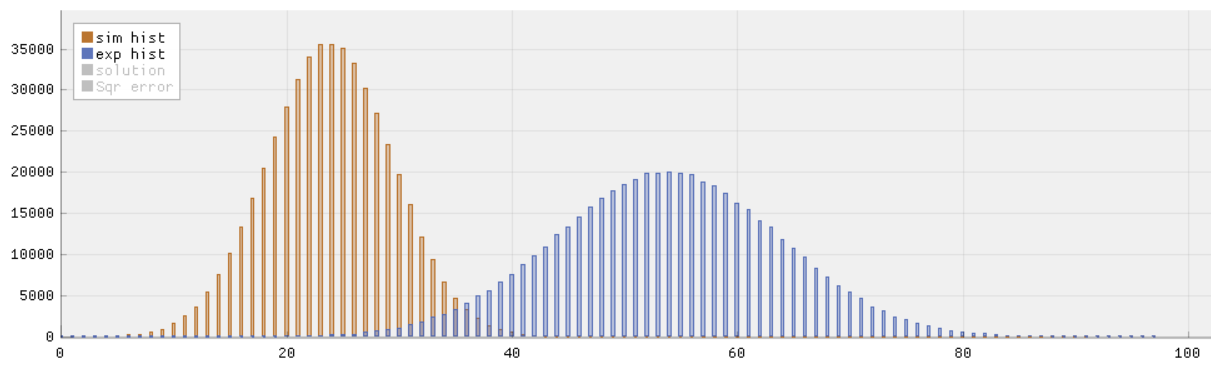
\includegraphics[width=\linewidth]{images/gaus_dist.png}
   \caption{Пример смещенного и сжатого вдвое истинного спектра \\
   Ось абсцисс - номер бина, ось ординат - количество элементов в бине }
   \label{photo:gaus_dist}
 \end{figure}

Мы генерируем распределение $\tau$ размерности $n_{\tau}$ в соответствии с некоторой идеей лежащего в основе физического процесса и 
выполняем моделирование нашего детектора. Для начала разделим множество значений исходной величины на интервалы 
$(\Delta_{1}, \Delta_{2}, \cdots ,\Delta_{n_{\tau}})$. Дискретным распределением величины будем называть вероятности попадания 
в определенный интервал $p = (p_{1}, p_{2}, \cdots, p_{n_{\tau}})$. Для разбиения множества истинных значений можно использовать 
другие интервалы $(\Delta'_{1}, \Delta'_{2}, \cdots ,\Delta'_{n_{m}})$, но в данной работе будет рассмотрен вариант с одинаковым 
биннингом для измеренных и истинных значений. Количество частиц, по итогам эксперимента детектированных аппаратурой в выделенных 
ячейках, обозначим $m = (m_{1}, m_{2}, \cdots, m_{n_{m}})$ и будем называть измеренным многомерным спектром. 


На этом этапе каждую запись в измеряемом бине (то есть каждое событие) можно напрямую проследить до ее происхождения. 
Это дает нам хорошо определенную систему линейных отношений между смоделированным истинным и измеренным распределениями: 
$A\tau = m$. Матрица $A$ размера $n_{m} \times n_{\tau}$ строится следующим образом, 
$A_{ij} = P( \text{ измеренное } \in \text{Bin}_{i} \mid \text{ истинное } \in \text{Bin}_{j} )$, 
то есть представляет собой вероятностную матрицу, которая фактически выполняет имитируемую процедуру свертки, обычно она называется матрицей
миграций или матрицей откликов.

Например, для случая изображенного на рис. \eqref{photo:gaus_dist} матрица миграций будет выглядеть следующим образом:

\begin{figure}[!ht]
   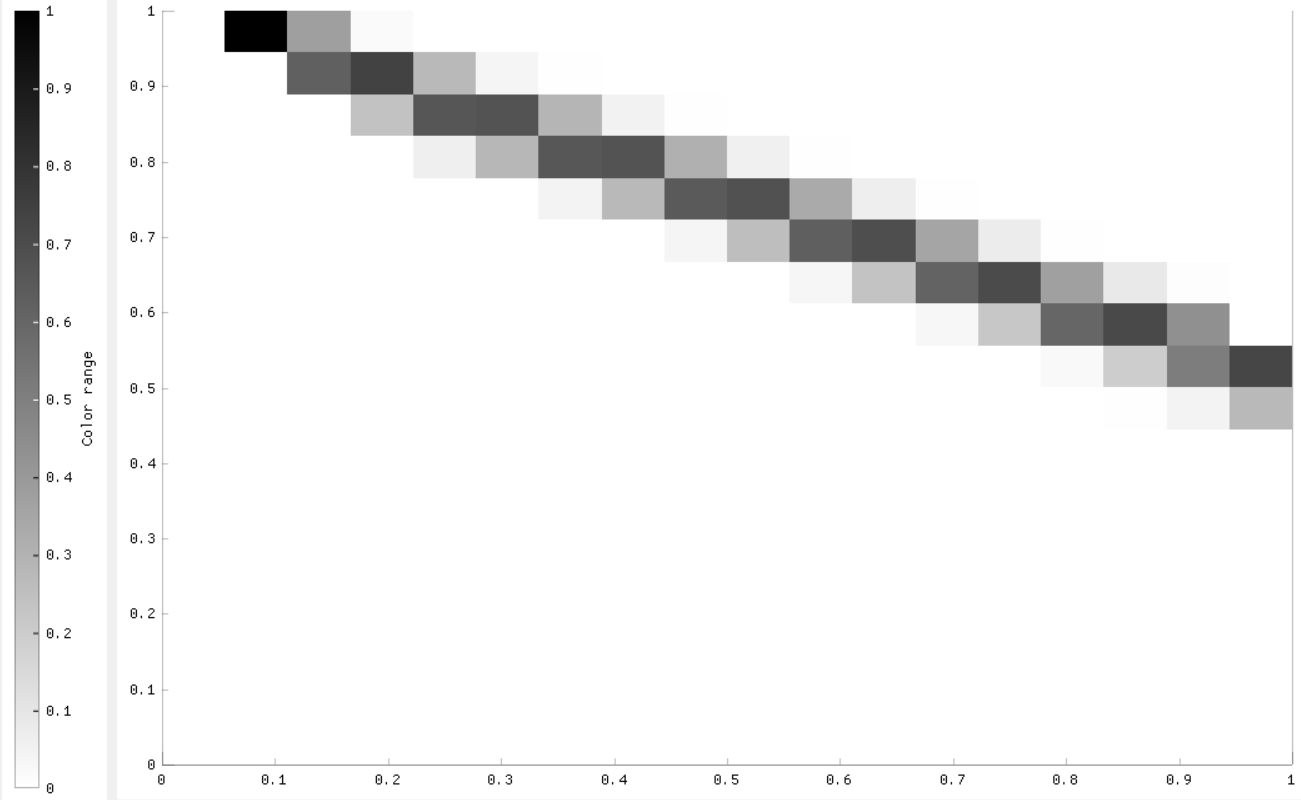
\includegraphics[width=\linewidth]{images/gaus_mig_black.png}
   \caption{Пример матрицы миграций распределения \\ изображенного на рис. \eqref{photo:gaus_dist} }
   \label{photo:gaus_mig}
\end{figure}

Данная матрица лежит не на главной диагонали, так как, в искажении присутствует сдвиг. При работе с данными физических частиц, 
матрица миграций чаще всего проходит через нее.

Непосредственное решение через инверсию матрицы $\tau = A^{-1} m$, обычно ведет к неприемлемым результатам, с большой статистической
ошибкой. Хотя сама оценка является состоятельной и несмещенной, но крайне чувствительной к небольшим колебаниям, что продемонстрировано 
в работе \cite{SvdHocker}, из-за чего не получится извлечь полезную информацию из решения задачи таким методом.


\subsection*{Методы решения задачи обратной свертки}

Существует несколько подходов для уменьшения статистических ошибок, которые являются доработкой прямого метода либо реализуют принципиально
новую идею решения задачи обратной свертки:
\begin{enumerate}
\item SVD-метод основанный на регуляризация Тихонова.
\item Байесовские методы (метод д’Агостини).
\item Метод поправочных коэффициентов.
\end{enumerate}

Далее рассмотрена модификация метода решения предложенного в работе \cite{SvdBogomolov}, основанная на идее регуляризации сингулярного разложения 
матриц. Данный подход интересен тем, что с его помощью можно использовать особенности, искомого спектра, отражая их в виде дополнительных функций, 
принимающих участие при решении задачи минимизации. Например, для регуляризации Тихонова, используется слагаемое, отражающее гладкость 
распределения, которое выражается через разность соседних линейно занумерованных бинов, для многомерного случая данный подход не работает, 
так как при переходе из многомерного в одномерный случай теряется информация о "многомерном" соседстве и после не учитывается при решении.

Оценку спектра истинных значений, которая была получена прямым методом, можно представить в виде точки минимума следующей функции: 

\begin{equation}
   \Phi(\tau)=(R\tau-m)^T (R\tau-m) \to min_{\tau}
   \label{min_base}
\end{equation}

Для того, чтобы учитывать дополнительно характер распределения, предлагается добавить регуляризационное слагаемое,  
которое может описывать, например, гладкость. С учетом дополнительного слагаемого система будет иметь следующий вид: 

\begin{equation}
   \Phi(\tau)=(R\tau-m)^T (R\tau-m) + \alpha S(\tau) \to min_{\tau}
   \label{min_svd}
\end{equation}
  
Здесь $S(\tau)$ как раз играет роль регуляризатора, а $\alpha$ - это коэффициент сглаживания. Соответственно при $\alpha = 0$ 
получаем исходную систему \eqref{min_base}. При таком подходе могут варьироваться количество дополнительных слагаемых и 
методы подбора коэффициентов. В данный работе берется за основу метод Картвелишвили и Хокера \cite{SvdHocker}, который подробно описан 
в следующих главах. 



\section{Сингулярное разложение матриц}

Для начала предлагается рассмотреть метод решения систем линейных уравнений, использующийся для последующего внедрения регуляризации.

Сингулярным разложение (или SVD) действительной матрицы $A$ размера $m \times n$ — это ее факторизация вида: 
\begin{equation}
    A = U S V^T 
    \label{svd_decomp}
\end{equation}

где $U$ — ортогональная матрица размера $m \times m$, $V$ — ортогональная матрица размера $n \times n$, а $S$ — диагональная матрица размера 
$m \times n$ с неотрицательными элементами на главной диагонали: 

\begin{equation}
    \begin{array}{l}
        U U^T = U^T U = I, \quad VV ^T = V^T V = I, \\
        S_{ij} = 0 \quad \text{ для } \ i \neq j, \quad S_{ii} = s_{i} \geq 0
    \end{array}
\end{equation}

Значения на главной диагонали матрицы $S - s_{i}$  называются сингулярными значениями матрицы $A$, а столбцы матриц $U$ и $V$ называются левыми 
и правыми сингулярными векторами. Сингулярные значения содержат очень ценную информацию о свойствах матрицы. Если, например, 
$A$ сама ортогональна, все ее сингулярные значения равны 1. Наоборот, вырожденная матрица будет иметь хотя бы один ноль среди своих 
сингулярных значений. Фактически ранг матрицы — это число ее ненулевых сингулярных значений. Если матрица линейной системы плохо обусловлена, 
а некоторые сингулярные значения матрицы значительно меньше других, система может быть трудной для решения, даже если формально матрица 
имеет полный ранг. Во многих аспектах такие матрицы ведут себя как вырожденные, и SVD предлагает метод решения таких проблем, который 
является общим для малых и нулевых сингулярных значений.

Будем считать, что сингулярные числа $s_{i}$ образуют невозрастающую последовательность, этого легко добиться, поменяв местами пары сингулярных 
значений, одновременно поменяв местами соответствующие столбцы $U$ и $V$. Предположим что $m \geq n$, это означает - 
количество бинов в измеренной гистограмме $m$ не должно быть меньше, чем количество бинов в предполагаемой истинной гистограмме $\tau$. 
При необходимости можно просто добавить строки нулей в исходную матрицу.




\section[Одномерный случай]{Решение задачи обратной свертки методом \\ регуляризации в одномерном случаии}

Для одномерного случая соседство определяется естественным образом, бины записываются последовательно, и соседними считаются, те бины, номер 
которых отличается на единицу. В качестве регуляризационного слагаемого из задачи минимизации \eqref{min_svd} предлагается брать следующую функцию:
\begin{equation}
    S(\tau)= \sum_{i=2}^{n-1} (\tau_{i-1} - 2\tau_{i} + \tau_{i+1})^2
\end{equation}

Которая отражает гладкость искомого распределения и является суммой квадратов второй производной по всем интервалам дискретизации. 
Она также может быть записана в матричном виде:
\begin{equation}
    S(\tau) = (C\tau)^T(C\tau)
\end{equation}
где матрица $C$ определяет соседство бинов и имеет следующий вид:

\begin{equation}
    C_{m,n} = 
 \begin{pmatrix}
   \quad 1 &       -1 &  \quad 0 &  \quad 0 & 0 & \cdots & 0 \\
        -1 &  \quad 2 &       -1 &  \quad 0 & 0 & \cdots & 0 \\
         0 &       -1 & \quad  2 &       -1 & 0 & \cdots & 0 \\
  \vdots &  & & \ddots & & & \vdots \\
  0  & 0  & 0 & 0 & \cdots & -1 & 1
 \end{pmatrix}
 \label{one_dim_neighbors_mat}
\end{equation}

Теперь мы можем переписать задачу минимизации \eqref{min_svd} следующих образом:

\begin{equation}
 \Phi(\tau)=(R\tau-m)^T (R\tau-m) + \alpha(C\tau)^T(C\tau) \to min_{\tau}
 \label{min_one_dim}
\end{equation}

Данную задачу минимизации можно переопределить в виде расширенной системы линейных уравнений:

\begin{equation}
    \begin{bmatrix}
        RC^{-1} \\
        \sqrt{a} \cdot I
    \end{bmatrix}
    C\tau = 
    \begin{bmatrix}
        m \\
        0
    \end{bmatrix}
    \label{system_one_dim}
\end{equation}

Здесь $I$ - значит единичная матрица. 
Точка минимума задачи \eqref{min_one_dim} будет достигаться при решении новой системы. Важно отметить что Матрица
$C$ - вырожденная, поэтому, для того, чтобы найти обратную матрицу следует ее возбудить, для этого ко всем элементам
на главной диагонали следует прибавить $\epsilon$, для определенности можно взять $10^{-3}$ или $10^{-4}$.

\begin{equation}
   C = C + \epsilon I
\end{equation}

Далее для решения системы воспользуемся описанным выше SVD алгоритмом \eqref{svd_decomp}. Для начала необходимо разложить 
матрицу $A$ на сингулярные составляющие, которая для переопределенной системы выглядит следующим образом:

\begin{equation}
   A =
   \begin{bmatrix}
      RC^{-1} \\
      \sqrt{a} \cdot I
  \end{bmatrix}
  C = USV^{T}
\end{equation}

После, следуя алгоритму, можно получить точное решения слау:

\begin{enumerate}
    \item Выполняем сингулярное разложение матрицы A \\
    $USV^T \tau = m.$

    \item Делаем замену $z = V^T\tau$. Получаем $USz = m.$

    \item $U$ - ортогональная, это значит, что обратная матрица равна транспонированной. Домножая систему на $U^{-1}$ получаем $Sz=U^Tm$.

    \item Далее делаем замену $d=U^Tm$, и система принимает вид $Sz=d$.

    \item Отсюда находим $z_{i} = d_{i} / s_{i}$. В матрице сингулярных значений, элементы находятся только на главной диагонали, 
    поэтому рассматриваем просто вектор $s$.

    \item Решение системы находим следующим образом $\tau = Vz$.
\end{enumerate}

При решение переопределенной системы, отличия будут при вычислении вектора $z$, теперь его значения будут вычисляться как:
$z_{i} = \frac{d_{i}}{s_{i}} \cdot \frac{s^2_{i}}{s^2_{i} + \alpha}$ (при $\alpha = 0$ решение системы
совпадает с решением \eqref{min_base}). Идейно можно представить это как фильтр, который пропускает низкие частоты, отсеивая слишком 
весомые растяжения.

\begin{figure}[h]
   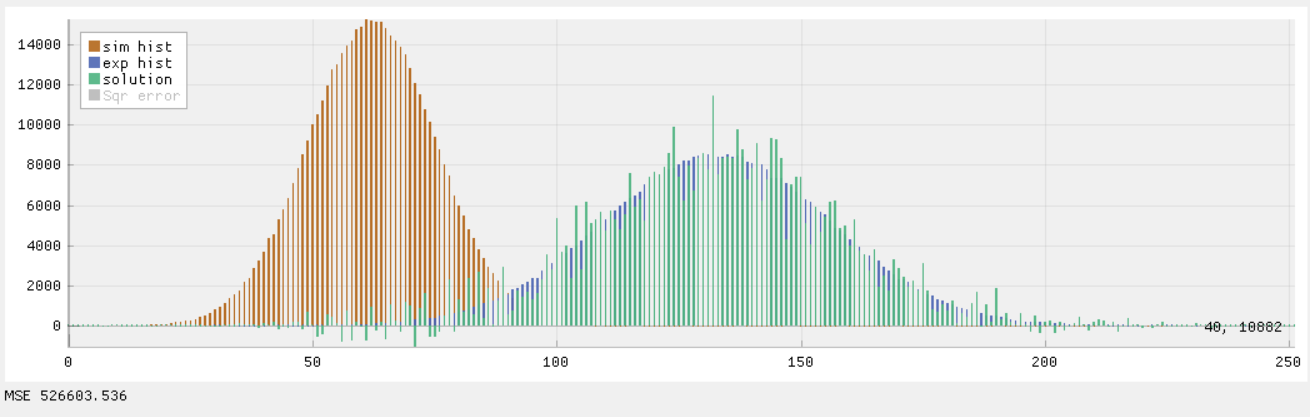
\includegraphics[width=\linewidth]{images/example_without_regulazation.png}
   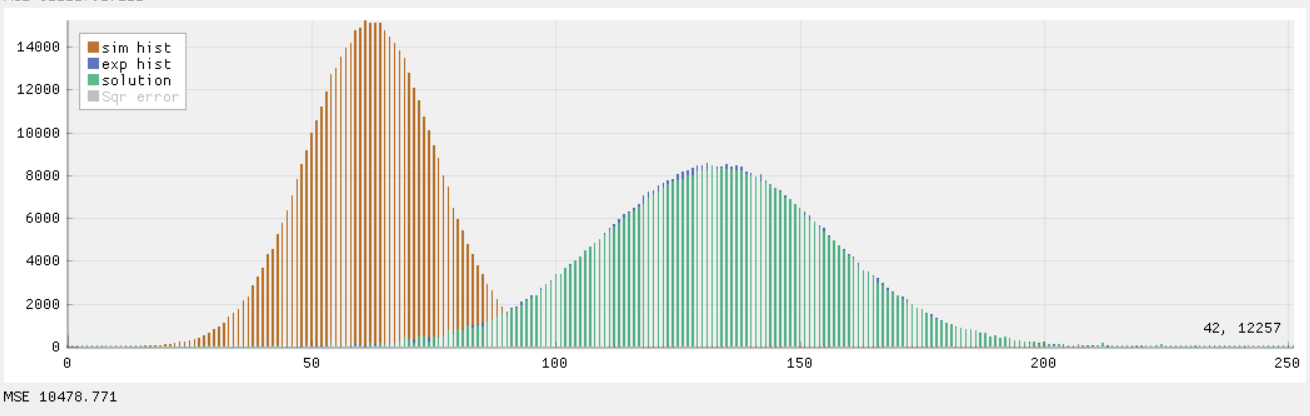
\includegraphics[width=\linewidth]{images/example_regulazation.png}
   \caption{Пример прямого решения и с использованием регуляризации}
\end{figure}

Данный алгоритм не зависит от регуляризационного слагаемого и может использоваться любое другое со схожей идеей. 
Например, в качестве функции регуляризации можно выбрать сумму квадратов оценок, других порядков или использовать формулы численного 
дифференцирования с более высоким уровнем погрешности.



\chapter{Решение задачи обратной свертки методом регуляризации в общем случаи}
\section[Многомерный случай]{Матрица Киргофа в качестве регуляризационного \\ слагаемого}

Для анализа физических частиц часто используются измерения нескольких параметров. Например, могут учитываться следующие величины: 
энергия, жесткость или различные углы входа частицы в прибор. Это значит, что задачу обратной свертки надо решать в многомерном 
случае. Сложность заключается в том, что матрица миграций описывает последовательно лежащие бины. Можно просто перевести задачу 
в одномерный случай, домножая последующие координаты на размерность первого пространства. Для дву-мерного случая $n$ $m$ переход 
будет выглядит как $n \cdot m$ - одномерный вектор. Как можно заметить, мы потеряли информацию о соседстве, для бинов, лежащих на
оси ординат. Это окажет существенное влияние на результат, так как, для регуляризации мы используем информацию о гладкости распределения и не 
сможем учесть ее относительно второго измерения.

Описанный в работе \cite{SvdBogomolov} метод, предлагает доработать регуляризационное слагаемое, которое позволит преодолеть проблему потери информации 
соседства многомерных бинов.

Рассмотрим следующую модификацию регуляризационной компоненты:

\begin{equation}
 k_{ij} =
  \begin{cases}
    deg(\Delta_{i}) & \quad \text{ при } i = j \\
     -1              & \quad i \neq j  \text{ , и } \Delta_{i} \Delta_{j} \text{- соседи } \\
\quad 0               & \quad \Delta_{i} \Delta_{j} \text{ - не являются соседними }
  \end{cases}
\end{equation}

Матрица $K = (k_{ij})$, или матрица Киргофа. Где $deg(\Delta_{i})$ отражает количество соседей $\Delta_{i}$. 
Как можно заметить, для одномерного случая матрица будет совпадать 
с $C$. При условии, что признак соседства описывает только бины, имеющие общие грани. 
Таким образом, решение можно назвать общим и дальше будем использовать его.

Из выше описанного следует, что матрица $C$ является подмножеством матрицы $K$, и для нового слагаемого можно вводить более сложные
отношения соседства. Во первых, близкими могут быть бины у которых не только общая грань, а во вторых, сила связи для разных бинов
может отличаться. Для силы связи введем параметр $\omega(\Delta_{i}, \Delta_{j}) \geq 0$ - который описывает вес соседних ячеек. 
Теперь постоим матрицу, с небинарным отношением:

\begin{equation}
 k_{ij} =
  \begin{cases}
    \displaystyle\sum_{k\neq i} w(\Delta_{i}, \Delta_{k}), \text{ при } \ i = j \\
    -w( \Delta_{i}, \Delta_{j} ), \text{ при } i \neq j
  \end{cases}
\end{equation}

И перейдем к финальной задаче минимизации:

\begin{equation}
   \Phi(\tau)=(R\tau-m)^T (R\tau-m) + \alpha(K\tau)^T(K\tau) \to min_{\tau}
   \label{min_n_dim}
\end{equation}
  

\section{Выбор параметра регуляризации}

В работе \cite{SvdHocker} предлагается подбирать параметр $\alpha$ на основе анализа сингулярных значений матрицы $A$. Сингулярные 
значения расположены в порядке убывания, этого мы можем добиться перестановкой строк и столбцов соответствующих матриц. Далее предлагается построить 
функцию $log$ для значений вектора:

% \clearpage
\begin{figure}[h]
   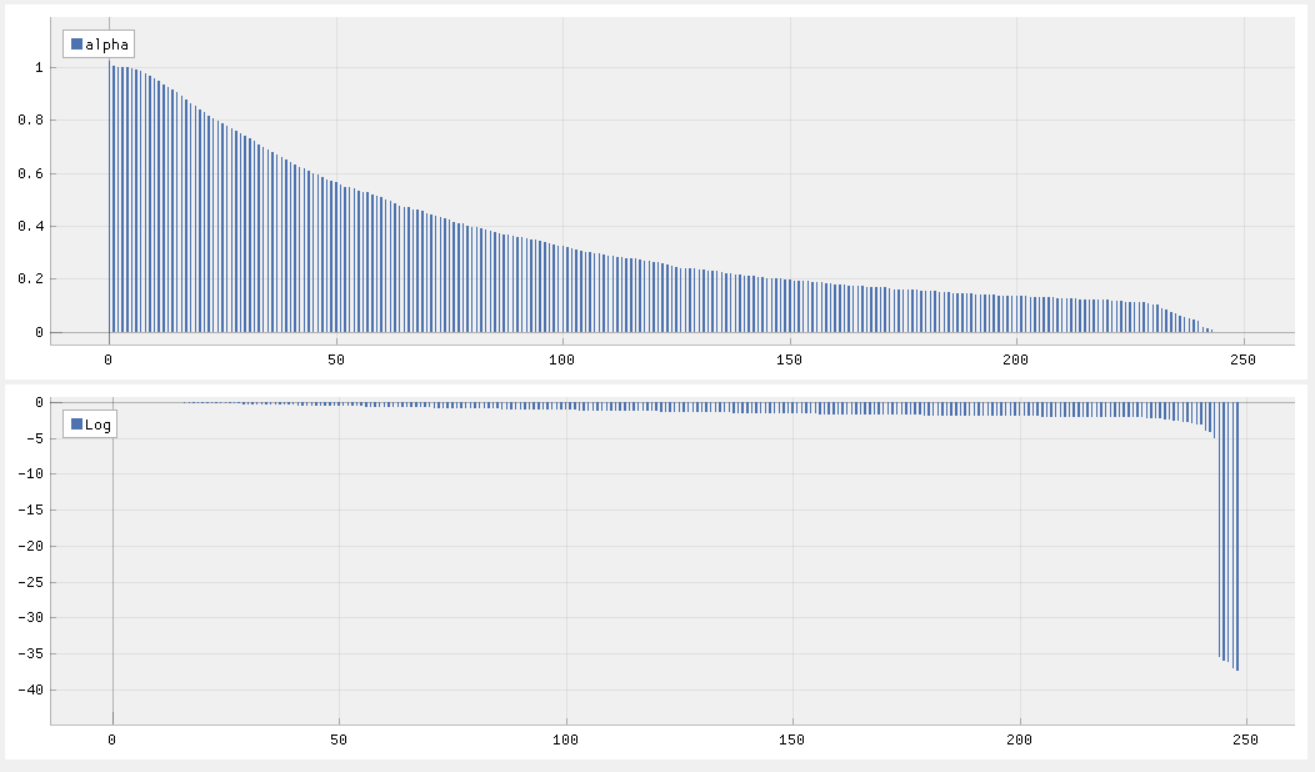
\includegraphics[width=\linewidth]{images/alpha.png}
   \caption{ Сингулярные значения матрицы $A$, и их логарифм }
   \label{photo:alpha}
\end{figure}

Можно заметить большой скачек в правой части, и основываясь на этих данных предлагается брать квадрат значения, сильно большего предыдущего или
$\alpha = s^2_{i}$ где $ s_{i} \gg s_{i+1} $. 
На графике логарифма, такое значение будет идти перед большим спадом.

На данных, рассматриваемых автором, данная оценка параметра, оказалась, почти точной, однако, при последовательном переборе, в окрестности 
находилось значение, при котором достигался лучший результат.

\section{Небинарные отношения соседства}

В данной секции автором были рассмотрены различные небинарные отношения соседства, для предложенной задачи \eqref{min_n_dim}, на данных 
предоставленных группой, которая занимается обработкой и изучением данных полученных прибором PAMELA в ходе эксперимента. Они представляют 
компьютерную симуляцию искажений спектра, полученного в системе Geant4. Каждая частица описывается тремя значениями, жесткость, полярный и 
азимутный углы. Собственно, в результате моделирования были получены пары истинных и измеренных значений, на которых и происходили замеры 
результатов решения задачи обратной свертки.

Вводя небинарное отношение соседства, легко заметить ограниченность метода \eqref{min_one_dim}. Во первых, как описано выше, бины могут 
быть близкими, например, большое число элементов истинного спектра попали в данный бин, и при этом они не имеют общих граней. Так же, 
связь соседних может оказаться сильнее, чем у других. За вычислением силы связи может стоять несколько идей: если мы, все же, 
считаем соседями бины с общими гранями, то можно учитывать площадь соприкосновения двух соседних бинов или их размеры. 
Более осмысленная идея, учитывать при вычислении силы связи расстояния центров масс бинов, в обратной пропорции. 
Данный подход более подробно описывает истинное распределение. Если центр масс 
тяготеет к оной из сторон, то мы получаем гораздо больше информации в сравнении с учетом только площади соприкосновения или размера интервалов. 

Следующая идея состоит в том, что мы считаем силу связи между $i$ и $j$ бином, на основании попавших в $j$-ый бин истинных значений при условии,
что измеренные попали в $i$ бин, соответственно, чем больше таких элементов, тем сильнее связь. При таком подходе удалось достичь наилучших 
результатов с наименьшей среднеквадратической ошибкой. Теперь более подробно рассмотрим построения и полученные результаты.

Построим матрицу соседства выполнив следующие шаги:

\begin{enumerate}
   \item  $k_{ij} = - count_(\Delta_{i}, \Delta_{j}) \cdot neighobrs(\Delta_{i}, \Delta_{j})$ \\

   \item  $k_{ii} = \displaystyle\sum_{j} k_{ij}$ \\

   \item  $k_{ij} = \frac{k_{ij}}{k_{ii}}$

\end{enumerate}

Где $count(\Delta_{i}, \Delta_{i})$ - функция, описывающая, количество истинных значений, попавших в $j$ бин. 
И $neighbors(\Delta_{i}, \Delta_{j})$ - функция, возвращающая 1, если два бина являются соседями и 0 в противном случае.

Важно отметить, при проверке на других данных, результат мог отличаться так же и в обратную сторону. Например, для распределения
представленного на рис. \ref{photo:gaus_dist}, бинарный случай оказался более результативным. А для данных, описывающих распределения жесткости
физической частицы, с использованием небинарной матрицы удалось достичь лучших значений.

Однозначный вывод для выбора матрицы соседства, на данном этапе, сделать невозможно. Для разных распределений может быть разный результат. 
Описывая выше несостоятельность некоторых идей для определения отношения соседства, автор делал выводы, исходя из результатов, полученных на 
конкретной задаче, и общего алгоритма подбора не было найдено.

Однако, можно описать некоторые возможные закономерности. Регуляризационное слагаемое \eqref{one_dim_neighbors_mat}, лучше себя показало на 
достаточно гладких данных, для таких, как у рис. \ref{photo:gaus_dist}. В то время, как подход, описанный в этой главе, проявил себя лучше в 
случаях резких переходов.


\chapter{Биннинг}
% \section{Бининг}

Бинниг или разбиение на интервалы множества значений непрерывной случайной величины оказывает существенное влияние на результат всего решения.
Для начала, бинниг может отличаться для истинного и измеренного спектров. Это необходимо для ситуаций, если оценки смещены относительно друг друга. 
На рис. \ref{photo:gaus_dist} изображен подобный случай.

В работе были рассмотрены следующие идеи для бининга:

\begin{enumerate}
   \item Статический биннинг ( разбиение области значений на равные интервалы ) \\
   
   \item Динамический биннинг ( Последовательно делим интервалы, с наибольшим числом элементов, 
   на два разных, проводя границу по центру исходного ) \\

   \item Динамический медианный биннинг ( Последовательно делим интервалы, с наибольшим числом элементов, 
   на два разных, проводя границу по медиане, то есть середине отсортированного вектора элементов )
\end{enumerate}


При дискретизации могут возникать проблемы с размером бинов, а именно, они могут оказаться слишком "высокими" или "широкими". При решении задачи 
обратной свертки польза, которую может принести решение такой задачи, будет мала. Первая часто возникающая проблема, это проблемы несостоятельных,
малых с точки зрения количества попавших частиц, бинов. 

Рассмотрим следующее распределение, описывающее жесткость частицы:

\begin{figure}[h!]
   \centering
   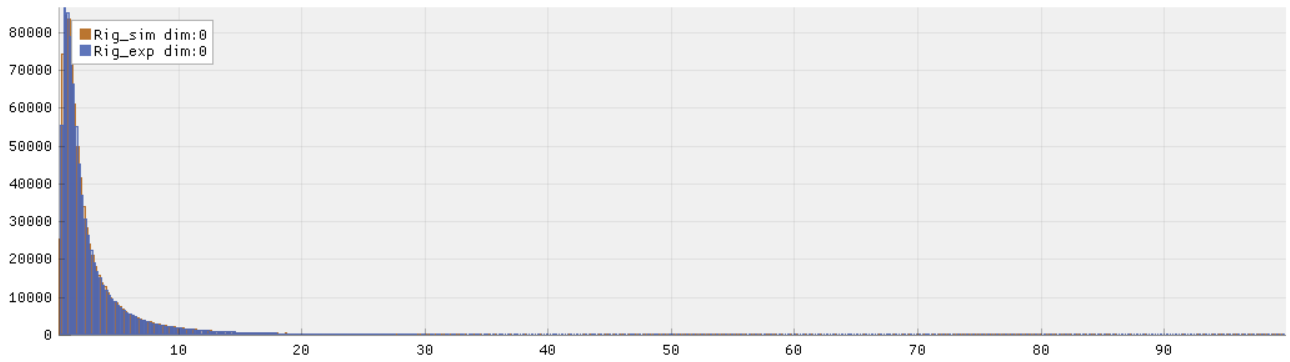
\includegraphics[width=\linewidth]{images/rig_dist.png}
   \caption{Гистограма для истинных и измеренных значений жесткости}
   \label{photo:rig_dist}
\end{figure}

Если мы разделим на равные интервалы относительно области возможных значений, мы получим разбиение следующего вида:

\clearpage

\begin{figure}[h!]
   \centering
   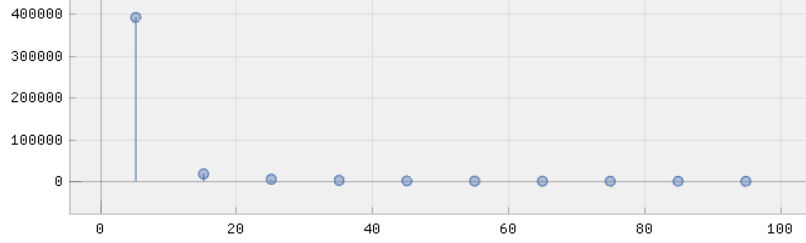
\includegraphics[width=\linewidth]{images/rig_static_binning.png}
   \caption{Пример статического биннинга}
   \label{fig:coffee}
\end{figure}

Здесь можно наблюдать сразу две проблемы. Первая - интервалы с малым количеством элементов. При нехватке информации для анализа, в результате
анфолдинга может возникнуть погрешность больше исходной. Так как количество элементов может существенно отличаться с тренировочной и тестовой 
выборке. Так же появился очень "высокий" бин, что также не желательно допускать при разбиении. При дроблении таких бинов можно получить более 
качественную оценку.

Динамический бинниг может являться альтернативным подходом разбиения, для подобного рода данных. Рассмотрим сразу динамический биннинг, 
основанный на делении пространства значений и делении на основе количества элементов.

 \begin{figure}[h!]
   \centering
   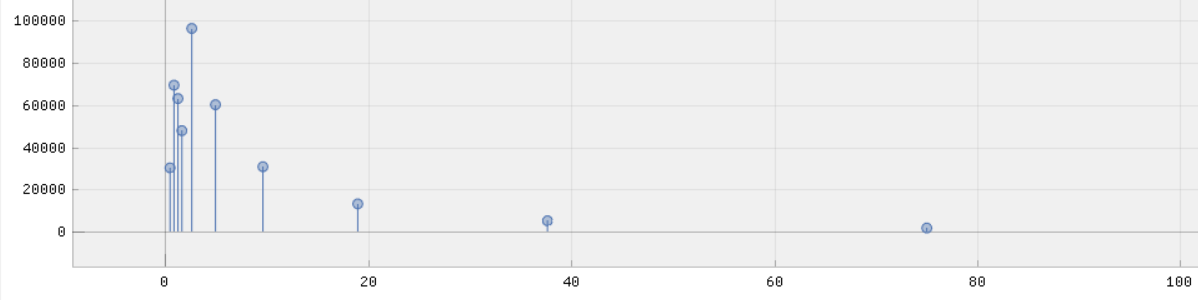
\includegraphics[width=\linewidth]{images/rig_dynamic_binning.png}
   \caption{Динамический биннинг}
 \end{figure}

 \begin{figure}[h!]
   \centering
   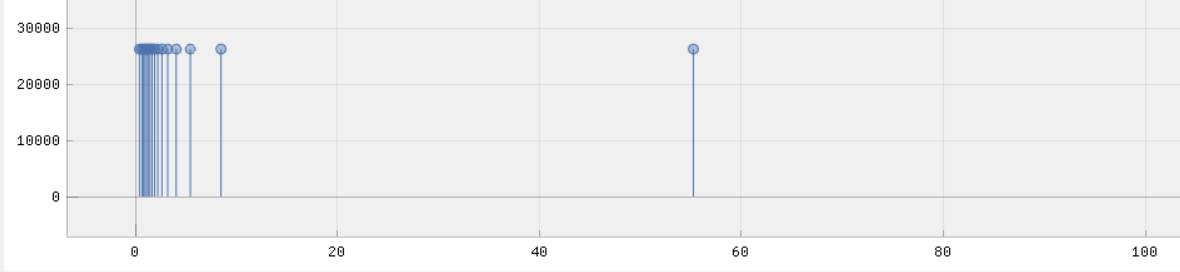
\includegraphics[width=\linewidth]{images/rig_median_binning.png}
   \caption{Медианный биннинг}
 \end{figure}
 

Здесь столбцы находятся на центрах бинов, об их размерах можно судить по расстоянию до соседа. Высота означает количество элементов в бине. 
Обе последние реализации справляются с задачей на порядок лучше стандартного подхода. Однако здесь становится видна вторая проблема биннинга.
На обоих примерах явно видно, что в конце остаются огромные по размеру бины. Почему же они являются не желательными. Для этого стоит вернуться к основной 
идее, которая заключаться в "отслеживании" переходов из одного бина в другой, и в последующем использовании этой информации для построения матрицы 
откликов. Имея настолько большие по площади интервалы, с высокой вероятностью можно утверждать, что переходов в соседний бин не будет, разве только,
что на краях интервала. Это ведет к бесполезности данной операции.

\begin{figure}[h!]
   \centering
   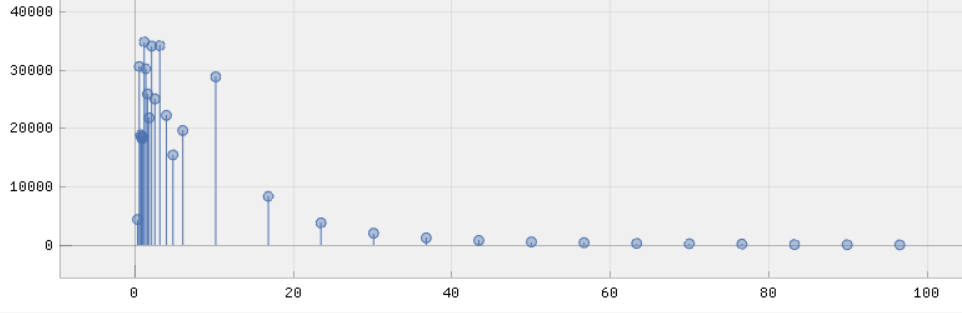
\includegraphics[width=\linewidth]{images/hybrid_binningpng.png}
   \caption{Гибридный биннинг}
   \label{photo:hybrid_binning}
\end{figure}

Последняя идея для построения интервалов совмещает в себе решение обеих проблем. Назовем ее гибридной, и она будет заключаться в том, что 
первую часть, например, половину интервалом мы получим статическим методом, а следующую часть достроим динамически. Таким образом, можно получить 
лучшее от обоих методов, а так же избежать их недостатков.

На данный момент биннинг является ручной работой, однако, рассматривая различные эвристические подходы, появилась идея о возможном точном решении 
данной задачи. Имея множество пар истинных и искаженных значений, требуется разделить множество значений на интервалы, с максимальным количеством 
пар, значения которых лежит в разных бинах. Представим пары в виде отрезков параллельных оси абсцисс, а бины прямыми параллельными оси ординат. 
Таким образом, лучшее разбиение можно представить, как решение следующей задачи - найти такие прямые, чтобы число пересечений было максимально, 
причем отрезки могут учитываться только при пересечении с одной прямой. Задачу можно записать следующим образом:

$n - $ отрезков (пар), $m - $ прямых (бинов)

\begin{equation}
   \begin{cases}
      Pair_{i} \cap Bin_{j} \\
      Pair_{i} \centernot\cap Bin_{k} \quad \text{ при } k \neq j
   \end{cases}
   \to max
\end{equation}

Также в ограничениях были учтены минимальный и максимальный размер бинов. Однако, результат при решении данной задачи оказался хуже, 
предложенных выше эвристических идей. Скорее всего существует более точная формализация данной задачи, которая позволит 
достичь наилучшего, однозначного разбиения на интервалы.

\section{Результаты}
C применением всех описанных выше идей удалось достичь следующих результатов. Разбиение на интервалы производилось автоматически.

Первый график отражает среднеквадратическое отклонение тренировочных данных. 
Второй график демонстрирует среднеквадратическое отклонение результата анфолдинга с тестовым истинным спектром. 
Для одномерного случая удалось уменьшить погрешность в 200 раз, а для двумерного в 4 раза.

\begin{figure}[h!]
   \centering
   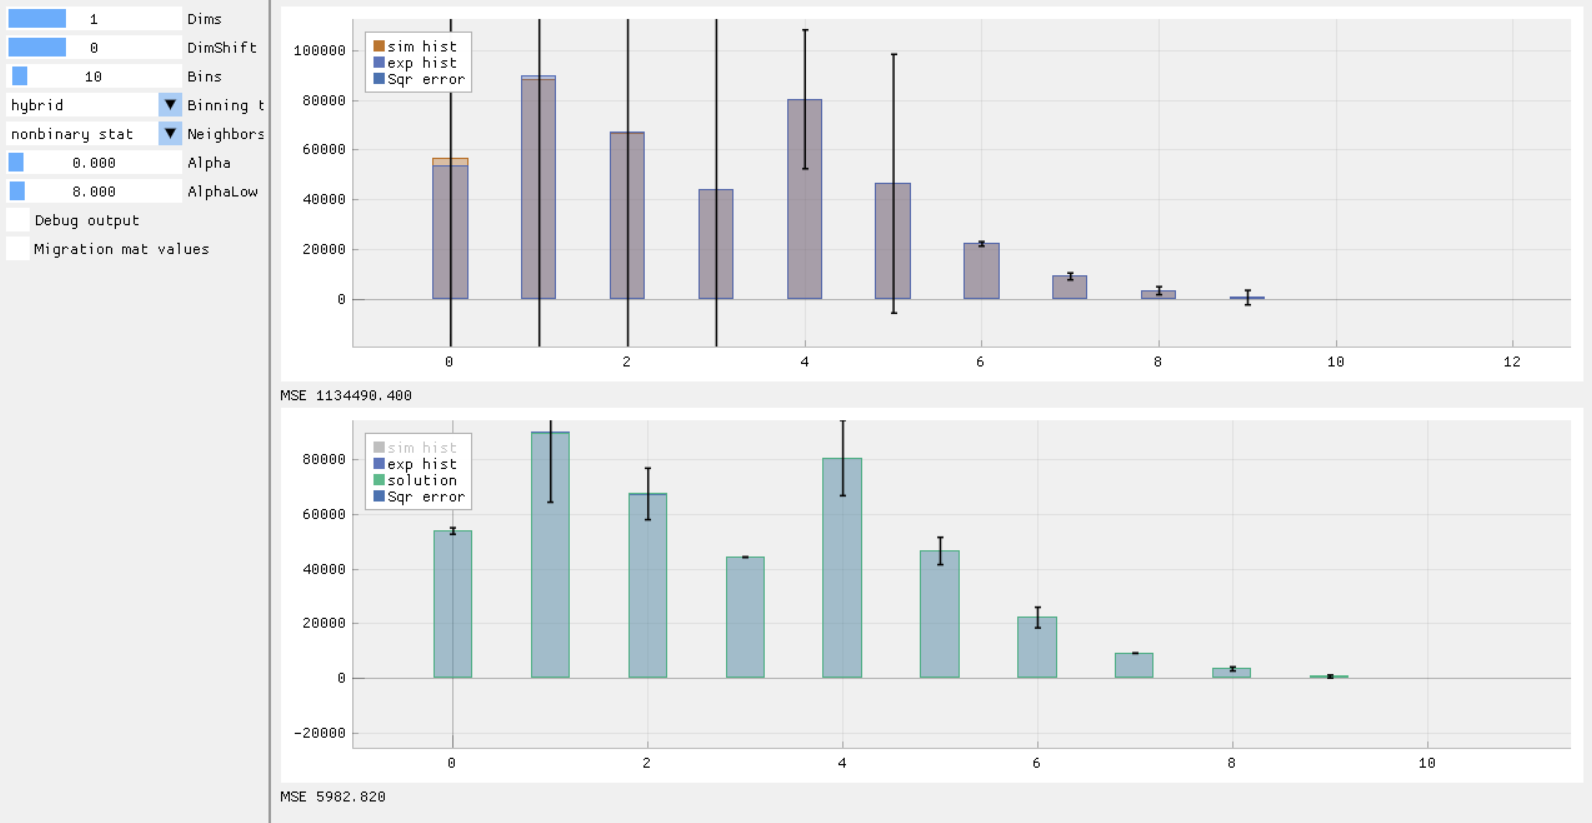
\includegraphics[scale=0.4]{images/1d_rig_res.png}
   \caption{Одномерный случай. Жесткость частицы}
\end{figure}

\begin{figure}[h!]
   \centering
   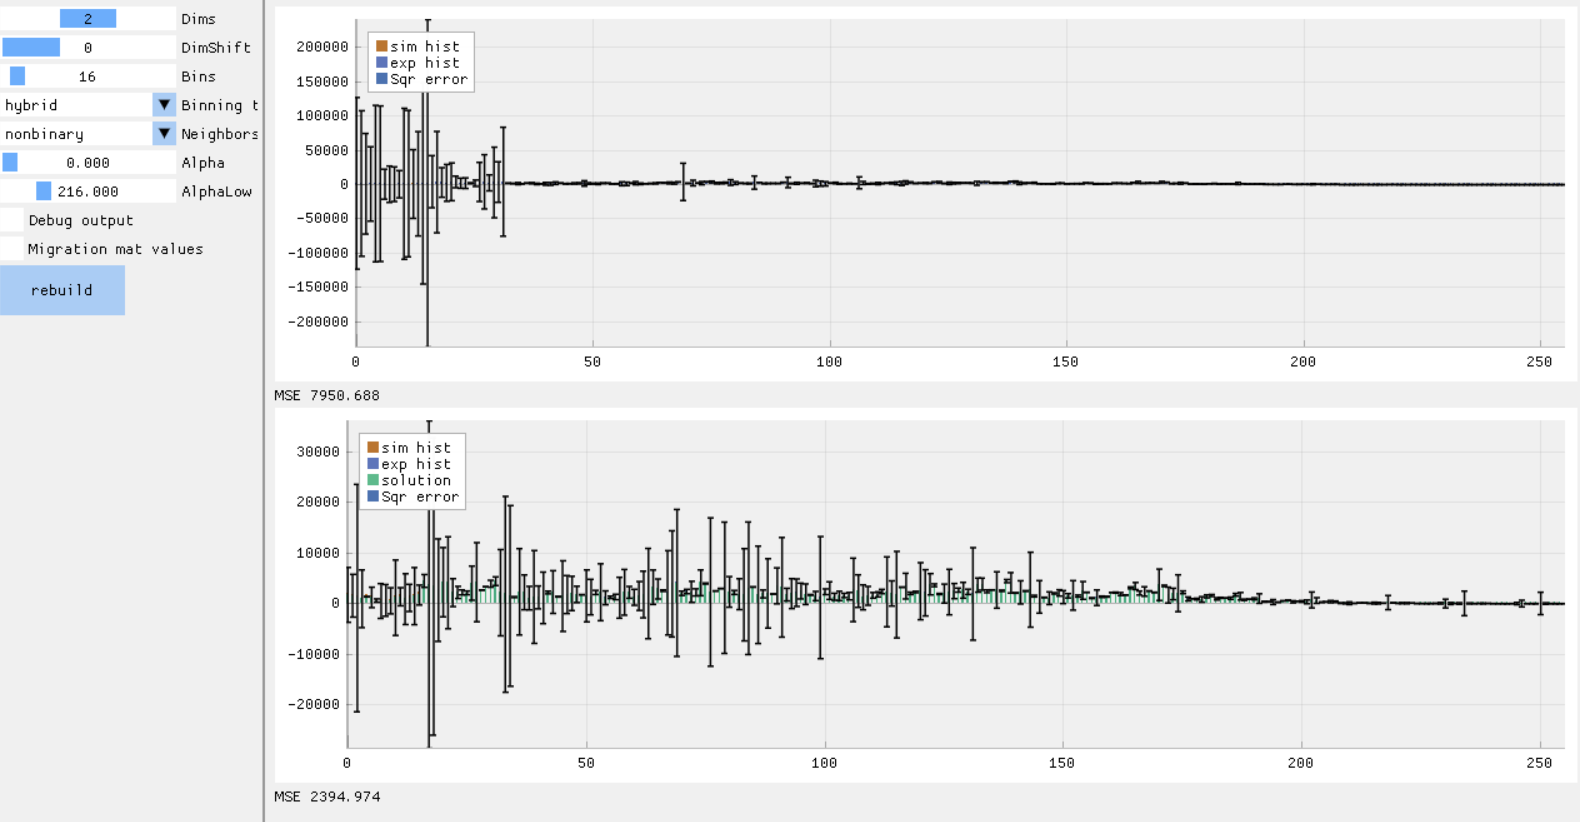
\includegraphics[scale=0.4]{images/2d_rig_azim_res.png}
   \caption{Двумерный случай. Жесткость и полярный угол}
\end{figure}


\chapternonum{Заключение}

В результате выполнения работы было разработано графическое приложение с использованием следующих инструментов. Был выбран язык программирование С++ для 
достижения максимальной производительности, так как, матрица миграций сама по себе являться квадратной от количества бинов, а количество самих 
бинов определяется степенной функцией от размерности пространства. Для отрисовки графики была использована связка библиотек SDL2 - для работы с 
окнами в операционной системе, ImGui и ImPlot для отрисовки пользовательского интерфейса и графиков. И наконец, для вычислений сингулярного 
разложения матриц была выбрана математическая библиотека alglib.

\begin{figure}[h!]
   \centering
   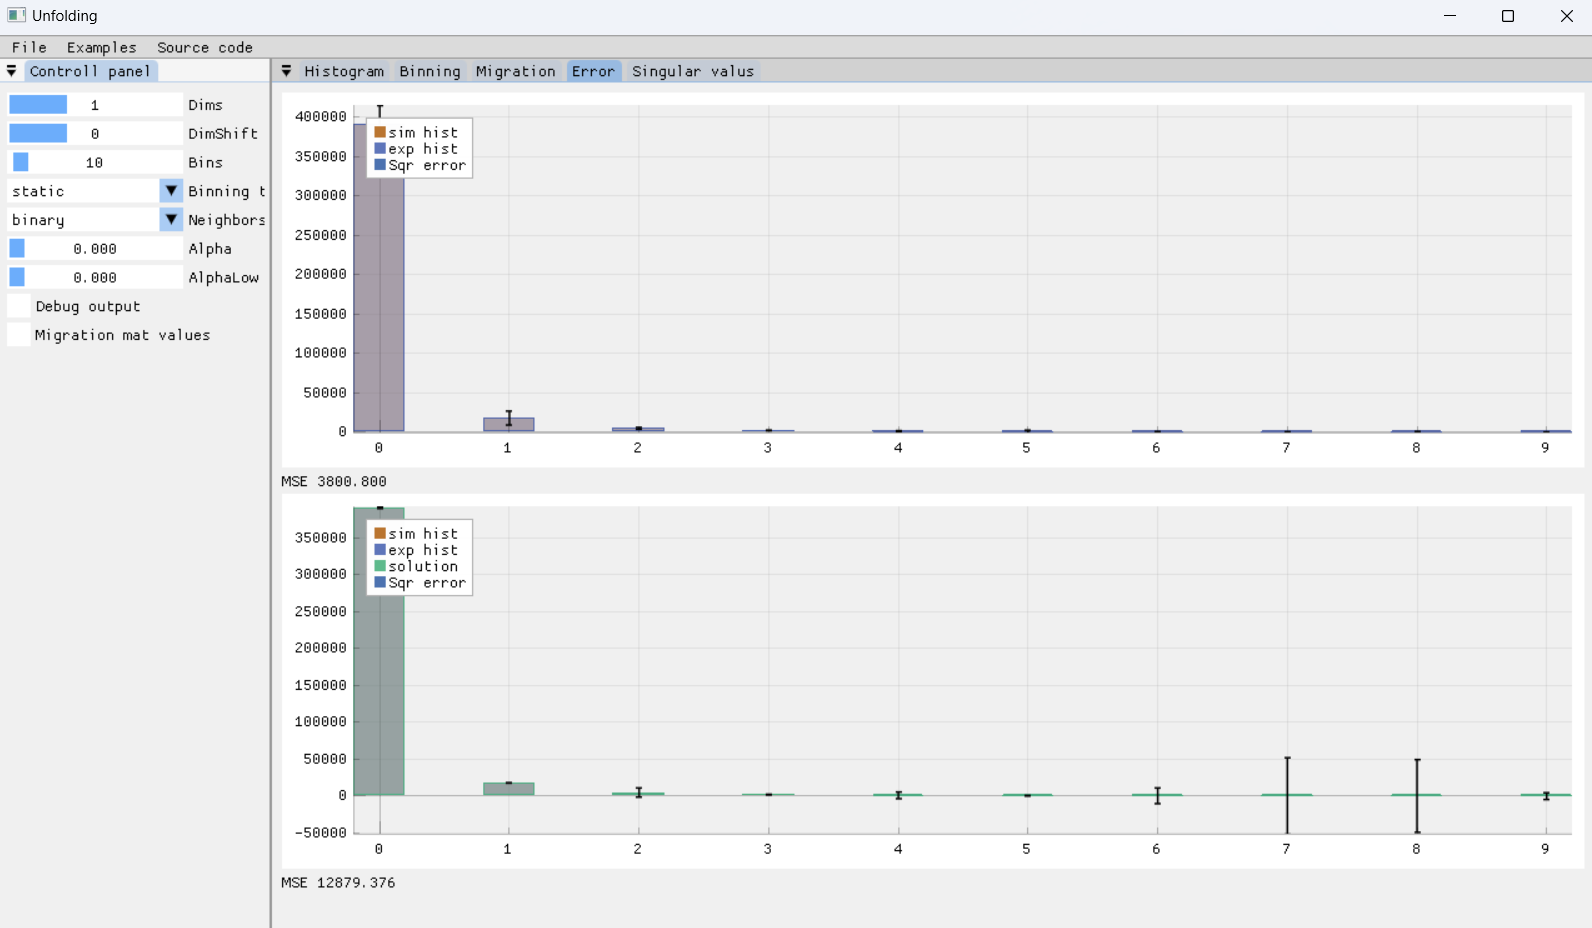
\includegraphics[width=\linewidth]{images/app_example.png}
   \caption{Разработанное приложение}
\end{figure}


С помощью данной программы можно в автоматическом режиме решать задачу обратной свертки,а так же отследить каждый шаг выполнения работы и полностью 
контролировать влияния тех или иных параметров. Например, без задержек оценить актуальность биннинга, с разными параметрами, основываясь 
на одномерных или двумерных проекциях, а так же на качестве матрицы миграций: 

\clearpage

\begin{figure}[h!]
   \centering
   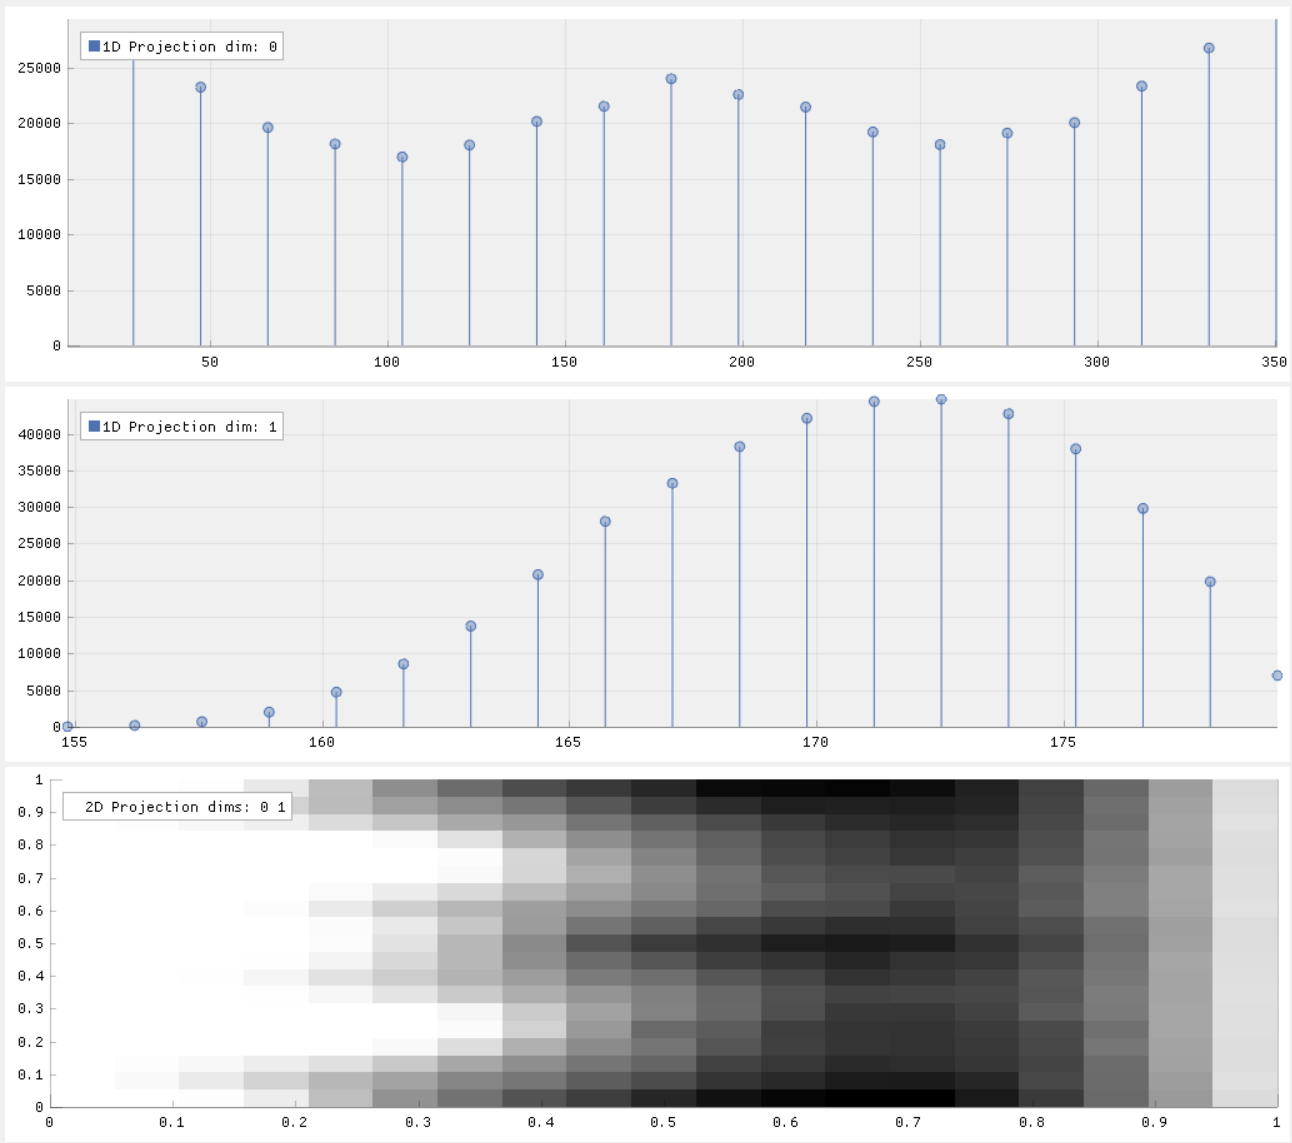
\includegraphics[width=\linewidth]{images/binning_projections_example.png}
   \caption{Одномерные и двумерная проекция}
\end{figure}

В результате проведенных работ было выяснено, что рассмотренные варианты для небинарных матриц не оказывают существенного влияния на 
результат, более того, в зависимости от данных и выбора отношения соседства разница может быть как и положительной, так и отрицательной. 

Было замечено, что разбиение на бины оказывает более весомый вклад в качество решения задачи. В зависимости от выбора интервалов, погрешность может 
сильно отличаться и даже быть выше, чем у исходных данных. Таким образом,  ё рассматривалась идея автоматизации процесса биннинга с помощью эвристических 
идей, а так же предложена идея алгоритма для точного решения данной задачи.



\begin{thebibliography}{9}

   \bibitem{SvdHocker}
     SVD Approach to Data Unfolding,
     Andreas Höcker, Vakhtang Kartvelishvili,
     1995.
   
   \bibitem{SvdBogomolov}
     Модификация регуляризационного SVD-метода обратной свёртки,
     Ю.В. Богомолов, В.В. Алексеев, О.А. Леванова, А.Г. Майоров, В.В. Малахов, С.Г. Язынин,
     Путь в науку,
     2022.

   \bibitem{UnfoldingMethods}
     Обзор методов обратной свертки,
     Ю.В. Богомолов, В.В. Алексеев, О.А. Леванова, А.Г. Майоров, В.В. Малахов, С.Г. Язынин,
     УСПЕХИ ФИЗИЧЕСКИХ НАУК ПРИБОРЫ И МЕТОДЫ ИССЛЕДОВАНИЙ,
     2022.

   \bibitem{ROOT}
      Официальный сайт пакета ROOT https://root.cern.ch/

   \bibitem{RooUnfold}
      Официальный сайт пакета RooUnfold \\ https://statisticalmethods.web.cern.ch/StatisticalMethods/unfolding/
   
   \bibitem{Schmitt}
      TUnfold, an algorithm for correcting migration effects in high energy physics,
      Schmitt S.,
      Journal of Instrumentation Vol. 7. No. 10,
      2012.

   \bibitem{Agostini}
      Improved iterative Bayesian unfolding,
      D'Agostini G.,
      arXiv preprint arXiv:1010.0632,
      2010.
   
\end{thebibliography}




% Приложения
\appendix
	
% Настраиваем общее для всех языков оформление листинга
\lstset{
	%	breaklines=true,
	%	frame=l,
	%	showstringspaces=false,
	tabsize=4, % длина табуляции в пробелах
	formfeed=\newpage, % реакция на символ "form feed"
	extendedchars=true, % используем неанглийские буквы
	basicstyle=\ttfamily, % базовый стиль
%	keywordstyle=\bfseries, % стиль ключевых слов (попробуйте \pmb если \bfseries не работает)
	commentstyle=\rmfamily\itshape, % стиль для комментариев
	stringstyle=\slshape, % стиль строк в кавычках
	numbers=left, % где проставляем номера строк; возможные значения: none, left, right
	numbersep=1em, % расстояние (по горизонтали) от номеров строк до кода
	stepnumber=1, % шаг отображения номеров строк. Если 1, то каждая строка помечается номером
	numberstyle=\footnotesize\color{black}, % стиль для номеров строк
}

% \chapter{Исходный код программы на C++}
% \label{app:source}

% Настраиваем оформление листинга для C++
% \lstdefinestyle{cpp}{
% 	language=[ANSI]C++,
% 	morekeywords={string, list} % расширяем список ключевых слов
% }

% Загружаем код из файла
% \lstinputlisting[style=cpp]{sort.cpp} 

% Части вашего текста можно хранить в отдельных файлах (это особенно удобно для приложений) и включать их в основной файл с помощью команды \input{имя файла}
% % !TeX encoding = windows-1251
% !TEX root = diplExample.tex

\chapter{Исходный код программы на Python}
\label{app:Python}

% Настраиваем оформление листинга для Python
\lstdefinestyle{Python}{
	language=Python,
	morekeywords={models, lambda, forms, self} % расширяем список ключевых слов
}

% Определяем ограничители для ввода меток на строки кода
% Для этого используем редкие для языка комбинации символов
\lstset{escapeinside={|@}{@|}}

Пример кода на Python 3 (взят с \href{http://python3.codes/alan-turings-automatic-machine/}{официального сайта}), реализующий симулятор машины Тьюринга для сложения унарных чисел (типа $11 + 111$).
Листинг позволяет делать (автоматическую) ссылку на какую"=нибудь строку. Например, на строку~\ref{lst:1} с командой \texttt{print(tape)}.

% Листинг кода на Python
%# Turing Machine simulator to add unary numbers (e.g. 11 + 111)
%#
\begin{lstlisting}[style=Python]
# prog is indexed by the current tape symbol (0 or 1) 
# and then by state (a kind of instruction pointer) 
# to get an 'instruction' comprising:
#   symbol to write on current tape position,
#   head action (-1 = move left, +1 = move right)
#   next state (like a goto jump).

#       symbol 0    symbol 1
prog = [[(1, +1, 1), (1, +1, 0)],         # state 0
		[(0, -1, 2), (1, +1, 1)],         # state 1
		[(0, +1, 2), (0, +1, 9)]]         # state 2
tape = [1,1,0,1,1,1,0,0,0]                # The data tape
head = 0                                  # head position on tape
state = 0                                 # instruction pointer
print(tape)  |@\label{lst:1}@|
while state != 9:                         # while not halt:
	symbol = tape[head]                   # read current tape symbol
	symbol, dir, state = t = prog[state][symbol] # lookup instruction
	print(' ' * (head * 3 + 1)+ '^  ' + str(t)) # display progress
	tape[head] = symbol                   # write new symbol on tape
	print(tape)
	head = head + dir                           # move tape head
\end{lstlisting}



% Конец документа
\end{document}
